\chapter{Modellarchitektur und Ablauf}

In diesem Kapitel werden die zwei Phasen bei SER, die Modellarchitektur und die Vorgehensweise des Frameworks bei einem SER-System erläutert. Hierbei können unterschiedliche Kalssifikationsverfahren verwendet werden, welche in 3.1  


\section{Zwei Phasen bei SER}

Die große Herausforderung für SER-Systemen ist die Unterscheidung der verschiedenen Emotionen durch die Sprache zu ermöglichen. Jeder Sprecher hat individuelle und kulturell bedingte Sprechstile, Sprechgeschwindigkeit, unterschiedliche Tonhöhe und Energiekontur im Spektrogramm, was das Extrahieren der Merkmale erschwert \cite{badshah2019deep}. Diese Umstände werden in der Verarbeitungseinheit behandelt, um später beim Klassifizieren der Sprachsignale bessere  Ergebnisse zu erhalten. 
\subsection{Verarbeitungseinheit (processing unit)}
Um die in 3.1 genannten Probleme anzugehen wird in der Verarbeitungseinheit das Spektrogramm in mehrere Blöcke (chunks) aufgeteilt, die Frames genannt werden (siehe Abbildung \ref{frames}) \cite{badshah2019deep}. Diese einzelnen Frames werden dann im nächsten Schritt Klassifikator) analysiert. 
\begin{figure}
	\centering
	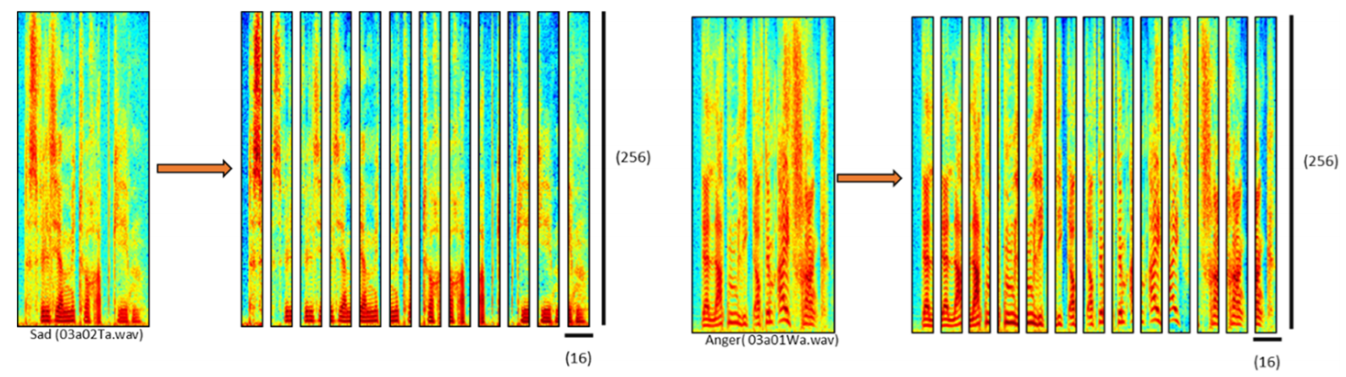
\includegraphics[width=1\textwidth]{images/frames}
	\caption{\label{frames}Spektrogramme, die in Frames aufgeteilt werden \cite{badshah2019deep}}
\end{figure}
\subsection{Klassifikator (classifier)}
Nachdem das Spektrogramm in mehreren Frames aufgeteilt wurde findet die Klassifikation mit Hilfe von Machine Learning Algorithmen statt \cite{badshah2019deep}. Hierbei werden die Frames einzeln untersucht und es können verschiedene Arten von Klassifikationsverfahren zum Einsatz kommen. Die gängigsten Algorithmen sind Hidden-Markov-Modelle (HMM), Gaußsches Mischungsmodell, Support Vector Machine (SVM), künstliche neuronale Netze und K-nearest neighbor, wobei SVM und HMM die am weitesten verbreitete Lernalgorithmen für sprachbezogene Anwendungen sind \cite{badshah2019deep}. \newline
\textbf{SVM} ist weit verbreitet für Mustererkennungs- und Klassifikationsprobleme \cite{svm}. Im Vergleich zu den anderen Klassifikationsverfahren ist der Vorteil bei diesem  Algorithmus, dass nicht so viele Traningsdaten benötigt werden um gute Klassifikationsleistung aufzuweisen \cite{svm}.
\newline
\textbf{HMM} ist ein statistischer Modellierungsverfahren, welcher bei Klassifikationsproblemen in Spracherkennungsanwendungen häufig eingesetzt werden \cite{HMM}. Die Grundidee bei HMM ist es, dass ein endliches Modell, welches einer Wahrscheinlichkeitsverteilung über eine unendliche Anzahl möglicher Folgen beschreibt.\cite{HMM}.

Wichtig ist es den Klassifikator zu trainieren. Dazu benötigt man gelabelte Datensätze, die als Tranings-Daten dienen. Hier bietet sich zum Beispiel die Emo-Db an \cite{burkhardt2005database}. In der Datenbank befinden sich gelabelte Tonaufnahmen von fünf weibliche und fünf männliche Schauspieler \cite{burkhardt2005database}. Die gelabelten Emotionen sind Ärger, neutral, Angst, Freude, Trauer, Ekel und Langeweile \cite{burkhardt2005database}. Nachdem der Klassifikator trainiert wurde können Testläufe durchlaufen werden, um die Richtigkeit und Robustheit der Vorhersagen des Modells zu testen \cite{elearning}.

\section{Aufbau der Modellarchitektur}
In Abbildung \ref{architektur} wird der genau Aufbau der Modellarchitektur dargestellt. Als Input (links) für das CNN dienen die Sprachsignale in Form von Spektrogrammen. Die Architektur hat insgesamt fünf convolutional layer, drei pooling layer und drei fully connected layer (rechts) \cite{badshah2019deep}. Der Ausgang des letzten fully connected layer wird dem Softmax-Klassifikator weitergegeben, welcher für die Berechnung der Ausgangswahrscheinlichkeit und der Zuordnung der jeweiligen Emotions-Klasse zuständig ist \cite{badshah2019deep}. 

\begin{figure}
    \centering
    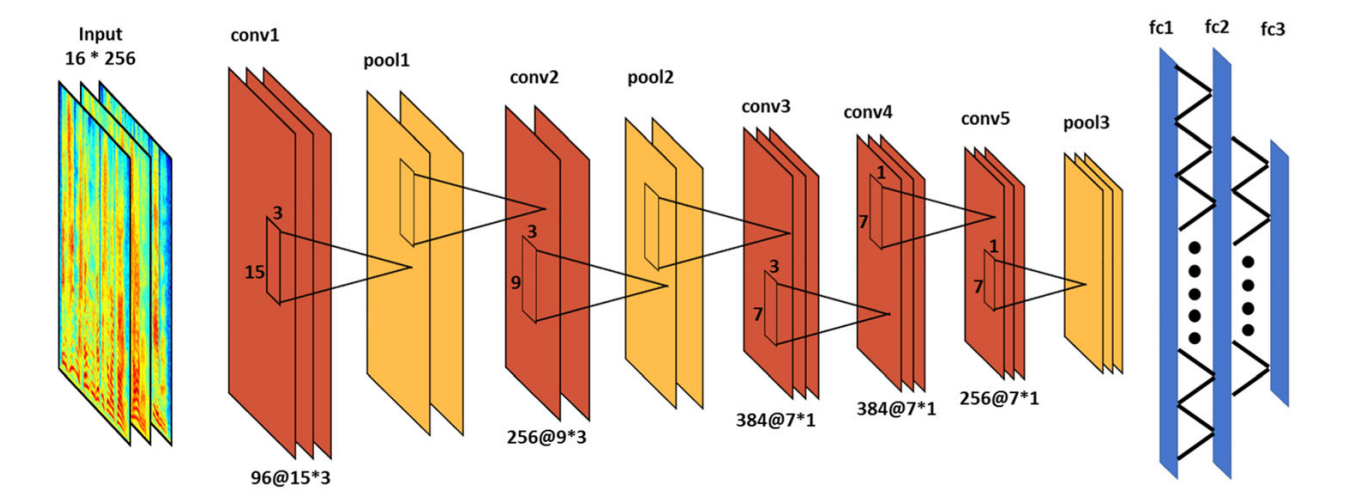
\includegraphics[width=1\textwidth]{images/conv}
    \caption{\label{architektur}CNN Architektur mit den unterschiedlichen Schichten \cite{badshah2019deep}}
\end{figure}


\section{Der Ablauf bei SER}
In Abbildung \ref{ablauf} ist der komplette Ablauf des SER-Systems abgebildet. Der Zyklus beginnt mit einem Audiosignal, welches durch STFT ein Spektrogramm erstellt wird. Dieses Spektrogramm wird im nächsten Schritt in Frames aufgeteilt. Dies ist die Verarbeitungseinheit des Inputes (siehe 3.1.1). Im nächsten Schritt werden die einzelnen Frames weitergeleitet an den Klassifikator, welcher 
\begin{figure}[ht]
	\centering
	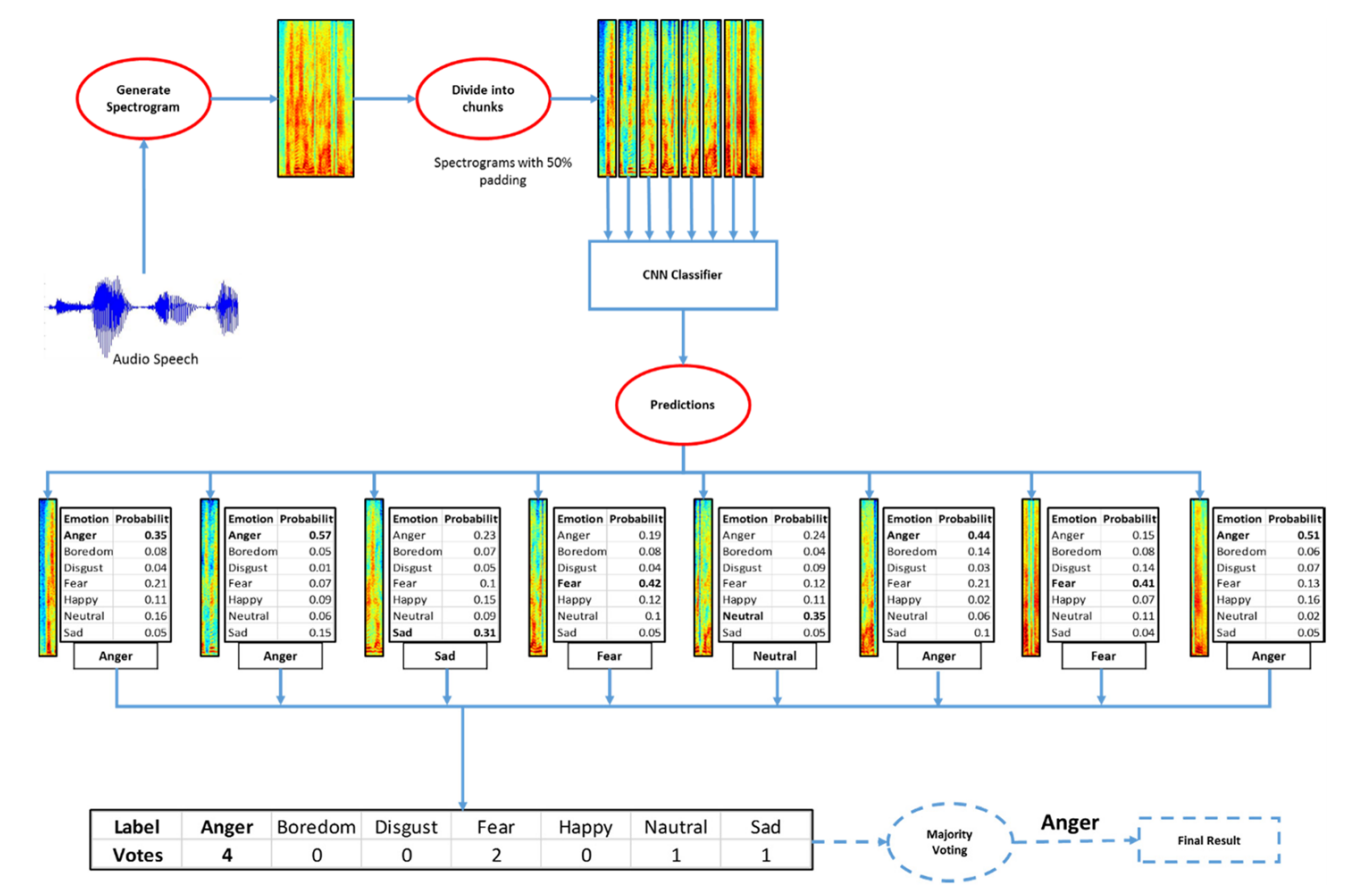
\includegraphics[width=1\textwidth]{images/ablauf}
	\caption{\label{ablauf}spezifischer Schema und Ablauf bei SER \cite{badshah2019deep}}
\end{figure}




